\documentclass{article}
\usepackage[T1]{fontenc}
\usepackage{lmodern}
\usepackage[a4paper, total={6in, 10in}]{geometry}
\usepackage{amsmath,amssymb}
\usepackage{graphicx}
\usepackage{booktabs}
\usepackage{xcolor}
\usepackage[colorlinks=true,linkcolor=blue!50!black,urlcolor=blue!50!black]{hyperref}

% Figures live in the lab root, one folder up from this file.
\graphicspath{{../}}

% Marks text that still needs filling in. Search for \fillme before submitting.
\newcommand{\fillme}[1]{\textcolor{red}{\textbf{[#1]}}}

\title{Computer Vision HS2026 -- Lab 02\\ \large Model Fitting \& Structure from Motion}
\author{Sebastian Banuelos}
\date{\today}

\begin{document}
\maketitle

% =====================================================================
\section*{1.6\quad Structure from Motion}

The reconstruction is initialized from images 0003 and 0004. The essential matrix between them
gives four possible relative poses. For each one, the matches are triangulated and only points with
positive depth ($Z > 0$) in both cameras are kept. The pose that keeps the most points is the
chosen one. Then, the remaining images are added one at a time, where their keypoints are matched to
keypoints that already have a 3D point. The resulting 2D-3D correspondences give the new camera
pose, and the new image is triangulated against all registered images to add more points.

Figure~\ref{fig:sfm-two} shows the initial reconstruction from the first two images;
Figure~\ref{fig:sfm-all} shows the final reconstruction after registering all images.

\begin{figure}[h!]
  \centering
  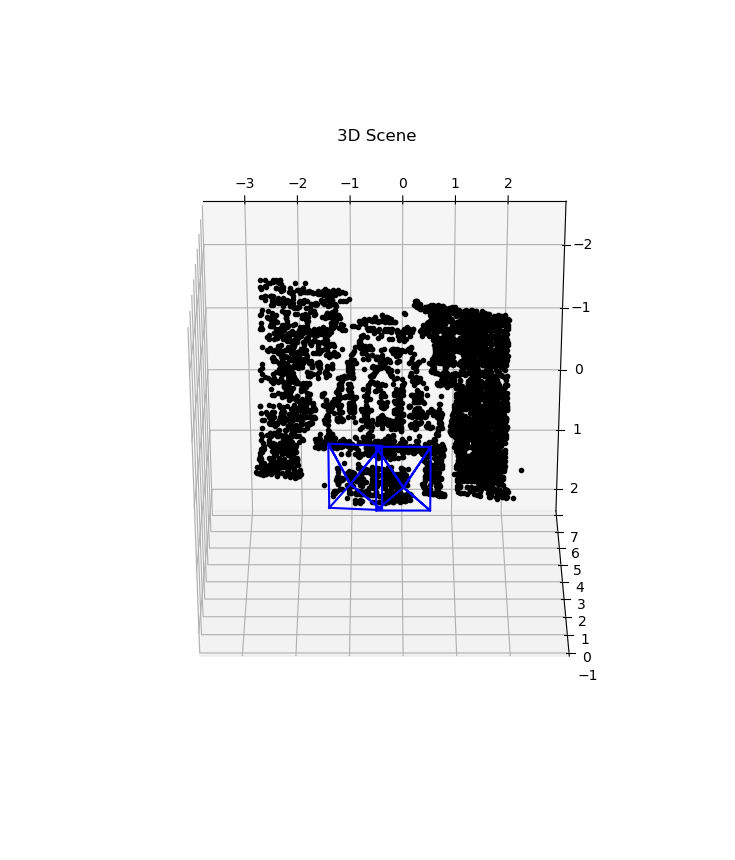
\includegraphics[width=0.62\linewidth, trim=126 122 91 84, clip]{reconstruction_2_frames.png}
  \caption{Two-camera reconstruction from the initial pair (0003, 0004). Only the part of the
  scene visible in both images is reconstructed.}
  \label{fig:sfm-two}
\end{figure}

\begin{figure}[h!]
  \centering
  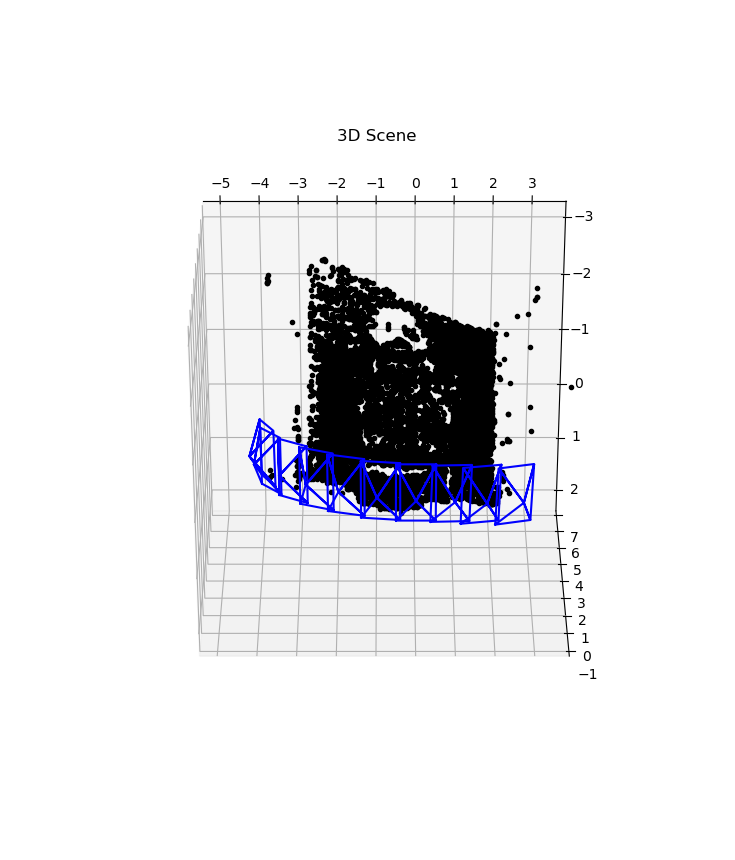
\includegraphics[width=0.62\linewidth, trim=126 122 91 84, clip]{reconstruction_all_frames.png}
  \caption{Final reconstruction with all 10 cameras (blue). The cameras lie on an arc in front
  of the object, and the added views extend the point cloud to the sides.}
  \label{fig:sfm-all}
\end{figure}

% =====================================================================
\clearpage
\section*{2.4\quad Model Fitting}

The data are 500 noisy points on $y = x + 10$. From this sample, 50 points are replaced by outliers.
Figure~\ref{fig:line} shows both fitted lines, and Table~\ref{tab:line} compares the
estimated parameters with the ground truth.

\begin{figure}[h!]
  \centering
  \IfFileExists{../line_fitting.png}{%
    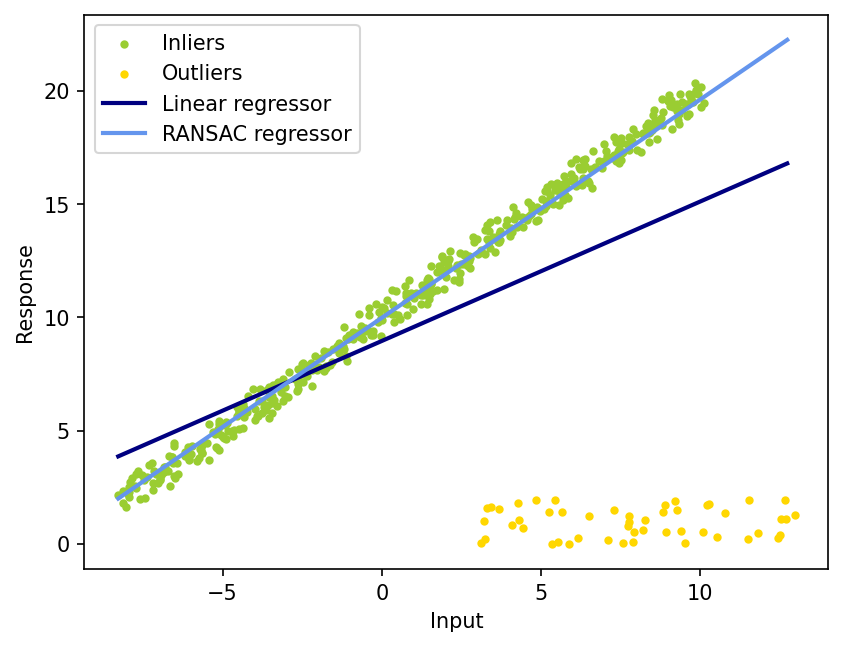
\includegraphics[width=0.75\linewidth]{line_fitting.png}%
  }{%
    \fbox{\parbox[c][5cm][c]{0.7\linewidth}{\centering
      \fillme{Save the line-fitting plot as \texttt{line\_fitting.png}\\ in the lab folder}}}%
  }
  \caption{Inliers, outliers, and the lines fitted by least squares and RANSAC.}
  \label{fig:line}
\end{figure}

\begin{table}[h!]
  \centering
  \begin{tabular}{lcc}
    \toprule
    & $k$ & $b$ \\
    \midrule
    Ground truth   & 1      & 10 \\
    Least squares  & 0.616  & 8.962 \\
    RANSAC         & 0.964  & 9.983 \\
    \bottomrule
  \end{tabular}
  \caption{Estimated line parameters.}
  \label{tab:line}
\end{table}

Least squares is pulled towards the cluster of outliers, because every point, including the outliers,
contributes to the squared error. On the other hand, RANSAC only considers candidate lines by how many points lie close
to them, so the outliers have little influence on its estimate.
We can observe RANSAC labels all 50 outliers correctly and its line runs through the
inliers only, while the least-squares line is visibly tilted towards the outlier cluster in the
lower right.

\end{document}
